\documentclass[12pt]{article}
\usepackage[a4paper, margin = 1in]{geometry}
\usepackage{amsmath, amssymb, graphicx, setspace}


\title{My First LaTeX Document}
\author{Baruuum}
\date{\today}

\doublespacing

\begin{document}

% generate title
\maketitle 
	
\section{Sociology?}

Why would you ever study sociology?

\begin{itemize}
	\item I have no idea
	\item Do you?
\end{itemize}

Why would you ever study mathematics?

\begin{enumerate}
	\item What is mathematics?
	\item Mathe...what??
\end{enumerate}

\subsection{Tables and Figures}

Table \ref{tab: freg} shows some fancy regression results. Nothing is significantly different from zero.

\begin{table}[h]
	
	\centering
	
	\caption{Fancy Regression Results}
	
	\begin{tabular}{lcr} \hline \hline
		coef. & s.e. & p \\ \hline
		Why & would & you \\
		ever & study & sociology? \\ \hline
	\end{tabular}
	
	\label{tab: freg}
	
\end{table}

Network plots like those in Figure \ref{fig: sbm} look super fancy, but are often misleading. 

\begin{figure}[h]
	\centering
	\caption{Some Fancy Network}
	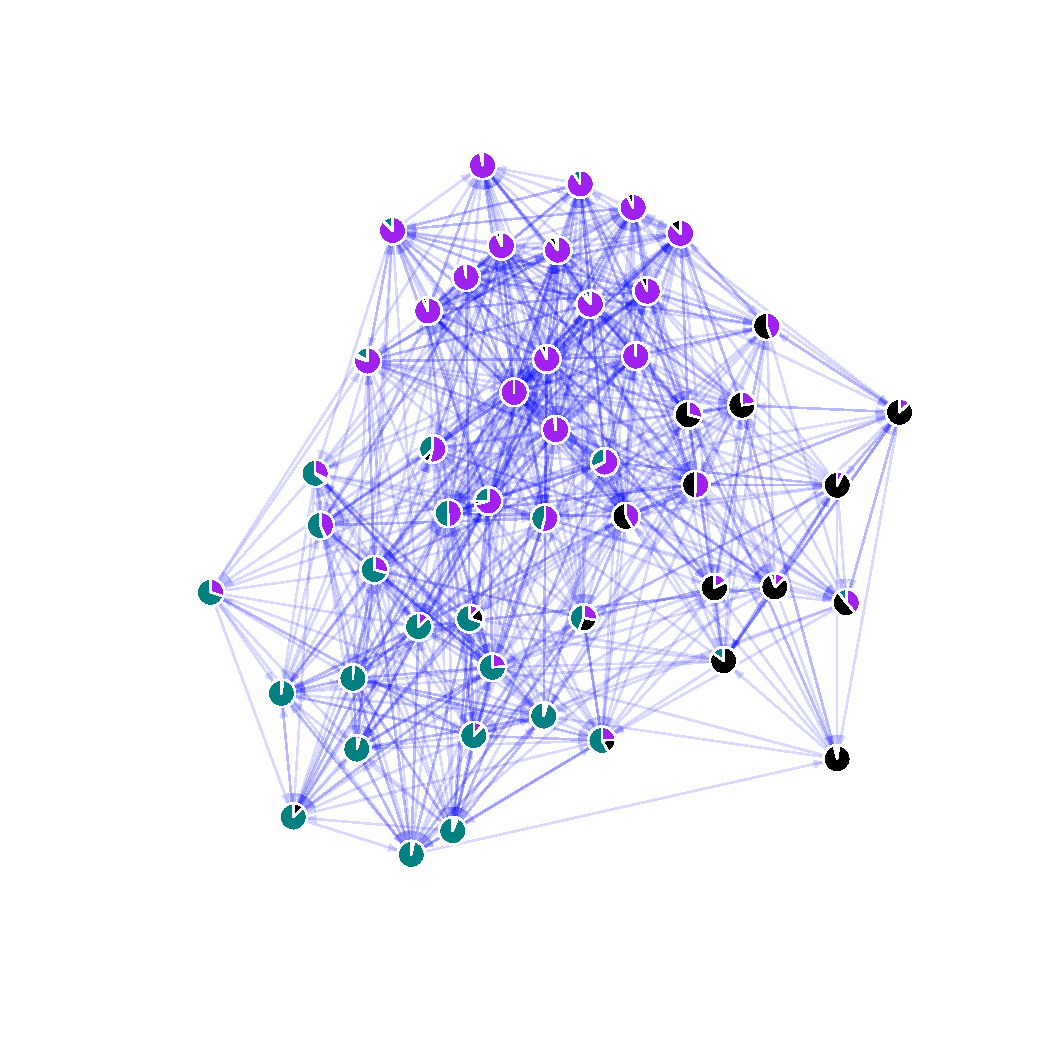
\includegraphics[width=.7\textwidth]{mmsbm.pdf}
	\label{fig: sbm}
\end{figure}

\section{Conclusion}

The expected value of a continuous random variable $X$ is $E[X] = \int_{-\infty}^\infty x f_{X}(x) dx$, given that it admits a density function $f_X$. Suppose $X$ has a standard normal distribution. Then it's density function is given as

\begin{equation}
f_X(x; \mu, \sigma^2) = \frac{1}{ \sqrt{ 2\pi \sigma^2 } } e^{-\frac{1}{2\sigma^2}(x-\mu)^2}.
\end{equation}

The expected value of the OLS estimator is
\begin{align*}
E[\hat\beta] &= E[(X'X)X'y] \\
&= (X'X)X'E[X\beta + \epsilon] \\
&= (X'X)X'X\beta + E[\epsilon] \\
&= \beta.
\end{align*}
Hence, it is unbiased.

\begin{center}
\Large Good luck with \LaTeX!
\end{center}
\end{document}
